\chapter{Brain structural connectivity}

The transfer of information and functional integration between different parts of the brain is influenced by white matter connections. The relationship between brain structure and function is still under active research, and the degree to which function is dependent on the structure is not entirely clear. However, there is no doubt that the relationship exists. In this work, we focus on the relationship between brain function, specifically its reaction to a stimulus, to the structure. 

Mapping billions of individual neurons in the human brain is intractable. Because of that, we attempt to use a simplified description of the structure while keeping its important properties. Structural connectome describes the structure of white matter fiber pathways as a graph. Vertices represent parts of the brain, and edges represent their anatomical connections. The connectome is usually represented as a connectivity (adjacency) matrix. \cite{yeh_mapping_2021}

The first section of this chapter describes the process of obtaining structural connectome. The following section is devoted to the specific connectomes used in this work.

\section{Structural connectome acquisition}

Structural connectome construction aims to give a macroscopic view of the brain structure. The problem consists of two parts. First, we have to define how to divide continuous grey matter into areas forming nodes. Second, we must estimate the length and \enquote{strength} of the white matter fiber bundles connecting these nodes to add weighted edges to the graph.

There are various approaches how to obtain structural connectome, both invasive and non-invasive. In this work, we consider diffusion-weighted magnetic resonance imaging (DW-MRI) and tractography, which is a non-invasive approach. It is an indirect method (it does not explicitly measure the quantity of interest), and because of that, it suffers from several limitations, extensively described in a paper The Seven Deadly Sins of Measuring Brain Structural Connectivity Using Diffusion MRI Streamlines Fibre-Tracking by Calamante et al. \cite{calamante_seven_2019}. Because of that, it is error-prone, and the results should be treated with caution. \cite{sotiropoulos_building_2019}

\subsection{Node definition using brain parcellation}

As described in Section~\ref{sec:MRI}, the result of the MRI is a 3D image. The next step is dividing continuous grey matter, represented by voxels in the 3D image, into a bearable number of discrete nodes. The resulting division is called parcellation, and the parcels/nodes are called regions of interest (ROI). 

The simplest and most common approach how to obtain brain parcellation is using one of the so-called anatomical atlases. An anatomical parcellation atlas is a standardized map of the brain based on anatomical features such as neural macrostructures (for example, sulci and gyri -- depressions or furrows and ridges on the cerebral cortex). Atlas-based image recognition works as follows: For a sample patient image, objects in the image can be recognized by registration of the sample image with the atlas image. By aligning corresponding points between the sample and atlas images, the labels assigned to regions in the atlas image can be transferred and applied to the sample image. \cite{sotiropoulos_building_2019, lawrence_standardizing_2021,chang_ljchangdartbrains_2020,rohrer_focused_2008} 

There are various parcellation atlases stemming from various a\-na\-to\-mi\-cal or functional perspectives. Created through a range of techniques, these parcellations enable various insights into the brain organization and network properties. However, the use of different parcellations across studies brings difficulties when comparing different studies and complicates reproducibility. The parcellations vary not only in the number of nodes but also in their positions. Because of that, results may vary; while one parcellation may reveal a particular effect, it might not be observable with another parcellation (see Section \ref{sec:ftract_dkt}). \cite{sotiropoulos_building_2019, lawrence_standardizing_2021}

Lawrence et al. made an effort to standardize the human brain parcellations in the Neuroparc project available on GitHub\footnote{\url{https://github.com/neurodata/neuroparc}}. For a nice summarization of various approaches to brain parcellation and a list of parcellation atlases, let us also recommend \textit{Introduction to Parcellations}\footnote{\url{https://dartbrains.org/content/Parcellations.html}, accessed 1. 5. 2024} by Sava-Segal and Botch (part of an online coursebook DartBrains by Luke Chang). \cite{chang_ljchangdartbrains_2020}

\subsubsection{Selected parcellations}\label{sec:parcellations}

We came across several parcellations while working with structural connectivity matrices. We provide their list, including short descriptions. 

\begin{itemize}
    \item \textbf{Yeo}\label{parc:Yeo} \cite{thomas_yeo_organization_2011}: The parcellation is based on the main functional areas in the brain and it was created using data from 1000 healthy subjects using a clustering approach. It divides the brain into 7 or 17 functional areas based on the version. We use the 7 networks version to color nodes of Schaefer parcellation (below) based on their functionality, see Figure \ref{fig:schaefer_colored_by_yeo}.

    \item \textbf{Schaefer200}\label{parc:Schaefer200}  \cite{schaefer_local-global_2018}: The parcellation is based on functional data from task-based fMRI and resting-state fMRI. There are several versions based on the level of detail, the number of parcels could range from 100 up to 1000. We used a version with 200 parcels. Each parcel also comes with Yeo's 7 Networks label.
    There is a parcellation is available on GitHub.\footnote{\url{https://github.com/ThomasYeoLab/CBIG/tree/master/stable_projects/brain_parcellation/Schaefer2018_LocalGlobal}}
\end{itemize}

\begin{figure}[!h]
  \begin{center}
    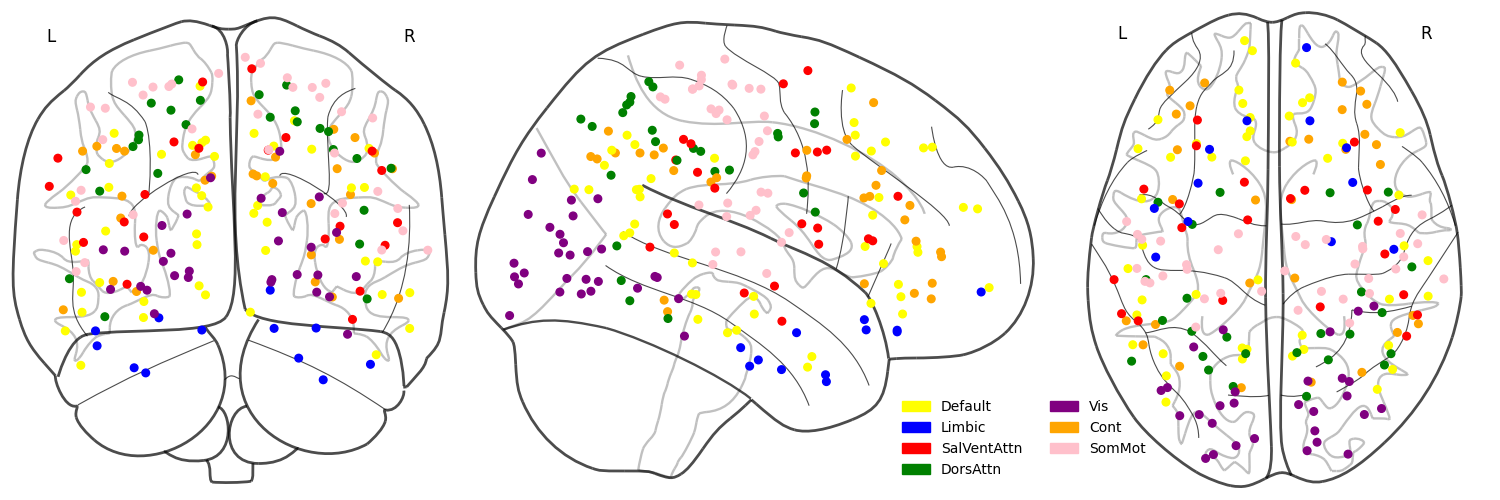
\includegraphics[width=\textwidth]{images/manually_created/Yeo7.png}
  \end{center}
  \caption[Schaefer200 centroids colored by Yeo7 networks]{Schaefer200 ROI centroids colored by Yeo7 networks.}
  \label{fig:schaefer_colored_by_yeo}
\end{figure}


\begin{itemize}
    \item \textbf{Desikan–Killiany (DK)}\label{parc:DK}  \cite{desikan_automated_2006}: The DK parcellation is defined by gyri. It was generated using 40 subjects (30 healthy and 10 with Alzheimer’s disease). It consists of 68 regions, 34 per hemisphere. There is also an updated Desikan-Killiany-Tourville (DKT) \cite{klein_101_2012} version of this parcellation, which merges regions that were not clearly defined. Because of that, DKT has only 62 regions. There is often confusion about which parcellation was used. We use only the version with 68 regions in this thesis, but the data sources sometimes mark it as DKT. Because of that, if the abbreviation DKT occurs, note that it also denotes Desikan–Killiany in our case.

    \item \textbf{Glasser}\label{parc:Glasser}  \cite{glasser_multi-modal_2016}: The parcellation is defined using a multimodal approach, combining brain anatomy (myelin content and cortical thickness), function (MRI measured during different tasks), connectivity (resting-state functional MRI) and topography. It is constructed based on data from 210 healthy subjects. It consists of 360 regions, 180 per hemisphere, which is the most detailed parcellation used in this work. It is sometimes denoted as MNI-HCP-MMP1.
\end{itemize}

In practice, we encountered several issues with parcellations usage. First of all, when we want to use a publicly available structural connectivity matrix, it is necessary to know not only which parcellation was used but also how the regions of interest are ordered in the matrix. Some authors use alphabetical ordering, while others use ordering based on the spatial proximity of the regions or their functional similarity. The main problem is that the paper does not always indicate the version. Therefore, we recommend being careful when using connectivity matrices from external resources.

Another problem was caused by the fact that the brain parcellation could use various coordinate systems.\footnote{Further information about coordinate spaces can be found in \textit{Coordinate Systems Appendix} of \textit{The Brain Imaging Data Structure} specification. The appendix is available on GitHub \url{https://github.com/bids-standard/bids-specification/blob/master/src/appendices/coordinate-systems.md} (accessed 1. 5. 2024). \cite{gorgolewski_brain_2016}} Because of that, it might be complicated to match data from two different resources even if they have the same parcellation.


\subsubsection{Node coordinates}

It is useful for the subsequent network analysis to keep the information about the spatial distances of the nodes. Because of that, we need to assign 3D coordinates to each node. The coordinates are obtained as a center of mass of the voxels registered as a part of the region of interest. They could be calculated for the atlas \enquote{model brain} or separately for each patient sample. For simplicity, we consider only the first option because we are working with average data, and the small differences are not of interest to us.

\subsection{Edges estimation}\label{sec:edge_estimation}

Conceptually, we want to create a map of long-range white matter fibers connecting the gray matter regions of interest discussed above. 

As explained in Section~\ref{sec:MRI}, DW-MRI measures water molecules' diffusion in brain tissues. It gives us information about the intravoxel axon arrangement. Based on this information (combined with some anatomical restrictions), a technique called tractography reconstructs the most probable streamline paths in white matter by tracing the water diffusion direction from voxel to voxel. \cite{yeh_mapping_2021,iturria-medina_characterizing_2007} 

The next step is defining a measure of connectivity between nodes. There are many options, such as the number, length, volume, or probability of streamlines between the corresponding nodes, but the mean value of a diffusion metric itself could also be used. \cite{yeh_mapping_2021} In this work, we use measures based on streamline counts and lengths because these were published by the authors of the connectivity matrices used here.

% https://commons.wikimedia.org/wiki/File:MRI_DWI_sequence_showing_restricted_diffusion_in_the_mesial_dorsal_thalami.jpg
% https://en.m.wikipedia.org/wiki/File:White_Matter_Connections_Obtained_with_MRI_Tractography.png

